% Lebenslauf DI Alexander Sommer  –  Stand Oktober 2026
% Compiler: pdfLaTeX (Overleaf-Standard). Foto als "foto.jpg" in das Projekt laden.
\documentclass[10.5pt]{article}
\usepackage[a4paper,top=16mm,bottom=16mm,left=18mm,right=18mm]{geometry}
\usepackage[T1]{fontenc}
\usepackage[utf8]{inputenc}
\usepackage[ngerman]{babel}
\IfFileExists{sourcesanspro.sty}%
  {\usepackage[default,semibold]{sourcesanspro}}%
  {\usepackage[scaled=0.92]{helvet}\renewcommand{\familydefault}{\sfdefault}}
\usepackage{microtype}
\usepackage{xcolor}
\usepackage{graphicx}
\usepackage{tabularx}
\usepackage{enumitem}
\usepackage{titlesec}
\usepackage{fancyhdr}
\usepackage{lastpage}
\usepackage[hidelinks]{hyperref}

\definecolor{accent}{HTML}{1F3A5F}
\definecolor{muted}{HTML}{5A6472}
\definecolor{rule}{HTML}{C9D1DB}

\hypersetup{pdftitle={Lebenslauf DI Alexander Sommer},pdfauthor={DI Alexander Sommer}}
\setlength{\parindent}{0pt}
\setlength{\parskip}{0pt}
\linespread{1.08}
\pagestyle{fancy}
\fancyhf{}
\renewcommand{\headrulewidth}{0pt}
\fancyfoot[L]{\footnotesize\color{muted}DI Alexander Sommer \,·\, Lebenslauf}
\fancyfoot[R]{\footnotesize\color{muted}Seite \thepage\ von \pageref{LastPage}}

% Abschnittsüberschrift: Versalien in Akzentfarbe, feine Linie
\titleformat{\section}{\large\bfseries\color{accent}}{}{0pt}{\MakeUppercase}[\vspace{-6pt}{\color{rule}\rule{\textwidth}{0.6pt}}]
\titlespacing*{\section}{0pt}{12pt}{6pt}

\setlist[itemize]{leftmargin=11pt,itemsep=1.5pt,topsep=2pt,label={\color{accent}\textbullet}}

% \entry{Zeitraum}{Rolle}{Organisation, Ort}{Inhalt}
\newcommand{\entry}[4]{%
  \begin{tabularx}{\textwidth}{@{}p{24mm}X@{}}
    {\leavevmode\small\color{muted}#1} & {\bfseries #2}\hfill{\small\color{muted}#3}\\[1pt]
    & \begin{minipage}[t]{\linewidth}#4\end{minipage}
  \end{tabularx}\par\vspace{5pt}}
% \kurz{Zeitraum}{Text} – einzeilige Station
\newcommand{\kurz}[2]{%
  \begin{tabularx}{\textwidth}{@{}p{24mm}X@{}}{\leavevmode\small\color{muted}#1} & #2\end{tabularx}\par\vspace{3pt}}
\newcommand{\kv}[2]{\textbf{#1} & #2\\}

\begin{document}

% ---------------------------------------------------------------- Kopf
\begin{minipage}[t]{0.70\textwidth}
  \vspace{0pt}
  {\fontsize{24}{28}\selectfont\bfseries\color{accent} DI Alexander Sommer}\\[4pt]
  {\large\color{muted} IT-Führungskraft \,|\, KI-Strategie \& Governance \,|\, Kritische Infrastruktur}\\[10pt]
  \small
  \begin{tabular}{@{}l@{\hspace{8pt}}l@{}}
    \kv{Adresse}{Gregorygasse 12/6/2, 1230 Wien}
    \kv{Telefon}{+43 681 102 104 17}
    \kv{E-Mail}{\href{mailto:alexander.sommer@gmail.com}{alexander.sommer@gmail.com}}
    \kv{LinkedIn}{\href{https://www.linkedin.com/in/sommeralex1982}{linkedin.com/in/sommeralex1982}}
    \kv{GitHub}{\href{https://github.com/sommeralex}{github.com/sommeralex}}
    \kv{Persönlich}{geb. 11.\,01.\,1982 in Wien \,·\, Österreich \,·\, verheiratet, 2 Kinder}
  \end{tabular}
\end{minipage}\hfill
\begin{minipage}[t]{0.25\textwidth}
  \vspace{0pt}\raggedleft
  \IfFileExists{foto.jpg}{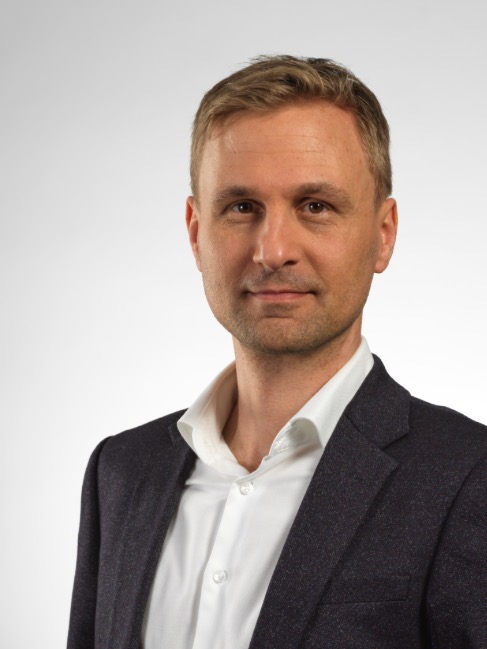
\includegraphics[width=36mm]{foto.jpg}}{\fbox{\parbox[c][36mm][c]{34mm}{\centering\color{muted}\small foto.jpg}}}
\end{minipage}

% ---------------------------------------------------------------- Profil
\section{Profil}
IT-Führungskraft mit mehr als 15 Jahren Erfahrung in Großunternehmen und kritischer Infrastruktur
(OMV, Wiener Wohnen, Austrian Power Grid). Verantwortet heute eine geschäftskritische
Applikationslandschaft mit mehr als 85 Systemen; zuvor die Harmonisierung von über 340
Corporate-Applikationen. Verbindet Führungs- und Governance-Erfahrung mit eigener,
nachweisbarer Entwicklungspraxis im Bereich Large Language Models (LLMs) und Agentic AI.
Leitgedanke ist der \emph{Digitale Humanismus}: Technologie wird daran gemessen, ob sie Menschen
entlastet -- nicht daran, wie viel sie automatisiert.

\vspace{6pt}
\begin{tabularx}{\textwidth}{@{}XXX@{}}
  \textbf{\color{accent}Führung \& Governance} & \textbf{\color{accent}KI \& Innovation} & \textbf{\color{accent}Wirkung}\\[1pt]
  \small IT-Strategie, Applikations-Portfolio, Vendor-Management, KRITIS-Compliance
  & \small Agentic AI, LLM-Integration, Model Context Protocol, Automatisierung (n8n)
  & \small bis 40.000\,EUR/Jahr Lizenzeinsparung; Einsparpotenzial bis 4\,Mio.\,EUR/Jahr strukturiert\\
\end{tabularx}

% ---------------------------------------------------------------- Werdegang
\section{Beruflicher Werdegang}

\entry{09/2025 -- heute}{Teamleiter Digital Workplace Solutions}{Austrian Power Grid AG, Wien}{%
\begin{itemize}
  \item Verantwortung für eine geschäftskritische Applikationslandschaft (Digital Workplace, mehr als 85 Systeme) im regulierten Umfeld kritischer Infrastruktur.
  \item Initiator und Leitung der Modernisierungsvorhaben \textbf{DMS 2.0} (Neuausrichtung des Dokumentenmanagements) und \textbf{Intranet NEU}.
  \item Kernmitglied des konzernweiten Veränderungsprogramms \emph{Change4Growth}; Themenverantwortung digitaler Arbeitsplatz (Digital Employee Experience).
  \item Innovation Peer: Pilotierung von Automatisierung (n8n) und KI-gestützter Softwareentwicklung im Unternehmenskontext.
\end{itemize}}

\entry{10/2022 -- 09/2025}{Teamleiter Corporate Applications}{Austrian Power Grid AG, Wien}{%
\begin{itemize}
  \item Steuerung, Absicherung und Harmonisierung einer Corporate-Applikationslandschaft mit mehr als 340 Systemen.
  \item Kostenreduktion von bis zu \textbf{40.000\,EUR pro Jahr} durch Konsolidierung und Lizenz-Governance (Adobe-Suite).
  \item Fachliche Teamführung, Steuerung externer Dienstleister; Gartner Technical Membership Account Holder.
\end{itemize}}

\entry{05/2020 -- 10/2022}{Leiter Digitalisierung \& Innovation}{Wiener Wohnen Kundenservice GmbH, Wien}{%
\begin{itemize}
  \item Gesamtverantwortung für Entwicklung und Umsetzung der Digitalisierungs- und Innovationsstrategie (Kundenservice, Hausbetreuung).
  \item Beratung der Geschäftsführung zu Technologiethemen; Gartner Executive Membership Account Holder.
  \item Verankerung des Leitgedankens „Technologie dient dem Menschen“ in der Strategie des kommunalen Unternehmens.
\end{itemize}}

\entry{10/2019 -- 05/2020}{Projektmanager Digitalisierung}{Wiener Wohnen Kundenservice GmbH, Wien}{%
Umsetzung zentraler IT-Projekte; Mitgestaltung der IT- und Innovationsstrategie.}

\entry{2018 -- 2019}{IT-Projektmanager Digitalisierung (Downstream)}{OMV Refining \& Marketing IT, Wien}{%
\begin{itemize}
  \item Globale Digitalisierungsprojekte in Retail, Raffinerie sowie Product Supply \& Sales.
  \item Identifikation und Strukturierung konzernweiter Einsparpotenziale von bis zu \textbf{4\,Mio.\,EUR pro Jahr}.
  \item Mitaufbau des OMV-Start-up-Ökosystems sowie der Mobile- und API-Strategie.
\end{itemize}}

\entry{2014 -- 2018}{IT-Projektmanager}{OMV Global Solutions, Wien}{%
\begin{itemize}
  \item Leitung von mehr als \textbf{40 internationalen IT-Projekten}, u.\,a. Rollout von Kassensystemen (ECR) und Outdoor Payment Terminals.
  \item Mitglied der Innovationsjury; Prototyping mobiler E-Commerce-Anwendungen für Großkunden.
\end{itemize}}

\entry{11/2011 -- 2014}{(Junior) Experte kurzfristige Optimierung}{OMV Downstream, Wien}{%
Integrierte, wertschöpfungsorientierte Optimierung über alle Raffinerien.}

\entry{01/2011 -- 10/2011}{Mobile Entwickler}{evolaris next level GmbH, Graz / Wien}{%
Anwendungsorientiertes Forschungs-Kompetenzzentrum (COMET/FFG). Konzeption und Entwicklung nativer mobiler Applikationen, u.\,a. der \emph{Raiffeisen Club Mobile App} (Loyalty, Couponing, Geo-Marketing) sowie Mitwirkung am durch Forschungsgelder geförderten Projekt \emph{»Sankt Onlein«} (Plattform für digitale Teilhabe; als Good-Practice-Initiative für IKT-Kompetenzen dokumentiert im \href{https://forschungsnetzwerk.ams.at/dam/jcr:0f8880c7-eb1b-4c50-aeca-1a61e2df9fbf/AMS_report_117.pdf}{AMS Report 117}).}

\entry{2008 -- 2010}{Network Operations}{Raiffeisen Informatik, Wien}{%
Netzwerkbetrieb. \textit{Davor:} OMV-Praktika 2001--2006 (Trading Support, Prozessoptimierung, IT-Support, Crude Planning).}

% ---------------------------------------------------------------- Unternehmertum
\section{Unternehmertum}
\kurz{2017 -- 2018}{\textbf{Co-Founder \& Projektmanager, Imovation} -- KI-basierte Healthcare-Services in Deutschland.}
\kurz{2013 -- 2018}{\textbf{Co-Founder \& Head Developer, 42Investors} -- regelbasierte, automatisierte Handelssysteme für NYSE/NASDAQ; Schwerpunkte Marktdatenverarbeitung, Risikoparameter und Systemstabilität im Live-Betrieb.}
\kurz{2018}{\textbf{Co-Founder, Goood Donation Platform} -- Patent für eine „private“ Kamera erhalten, Entwicklung gefördert durch die FFG.}
\kurz{2008}{\textbf{Gründer, Airwriting} -- in Kooperation mit HyperCMS GmbH.}

% ---------------------------------------------------------------- Repos
\section{Eigene Entwicklungspraxis}
{\small\color{muted}Neben der strategischen Führungsrolle bleibt eigenes, praktisches Verständnis neuer Technologien
wichtig. Die folgenden Projekte entstanden in Eigeninitiative; Code auf Anfrage einsehbar.\par}
\vspace{6pt}

\entry{seit 2025}{Peacethinking.ai -- Forschungsprojekt zu KI-gestützter Konfliktlösung}{Initiator \& Lead Developer}{%
Eigeninitiiertes Forschungsprojekt: Wie kann KI Menschen in Konflikten zu tragfähigen Einigungen begleiten -- nachvollziehbar, über fest definierte Abläufe statt freier Textgenerierung. Umgesetzt als Monorepo mit Web-, Mobile- und Desktop-Client, anbieterunabhängigem LLM-Gateway und DSGVO-orientierter Architektur (lokale Datenhaltung als Option, mehrsprachig). Reifegrad eines Forschungsprototyps.}

\entry{2026}{Excel-Reifecheck -- Datenqualität vor KI-Einsatz}{Python · WebAssembly}{%
Prüft Excel-Dateien auf Muster, die eine saubere KI-Weiterverarbeitung verhindern (verbundene Zellen, versteckte Farblogik, Magic Numbers). Die Analyse läuft vollständig im Browser, die Datei verlässt dabei nie das Gerät -- ein praktisches Beispiel dafür, wie sich Datenschutzanforderungen technisch statt nur organisatorisch umsetzen lassen.}

\entry{2025}{Simulationen \& Agenten-Prototypen}{HTML/JS · Python}{%
Kleinere Prototypen zur Veranschaulichung von Management-Fragestellungen (u.\,a. Business Case automatisierter Entscheidungsunterstützung) sowie ein KI-Agent zur regelbasierten Budgetklassifizierung (Opex/Capex) im Rahmen des MIT-Kurses \emph{Applied Agentic AI}.}

% ---------------------------------------------------------------- Ausbildung
\section{Ausbildung}
\kurz{2002 -- 2010}{\textbf{Technische Universität Wien} -- Wirtschaftsinformatik, Abschluss BSc und DI (beide Abschlussarbeiten mit „sehr gut“ bewertet und publiziert).}
\kurz{2000 -- 2001}{\textbf{Universität Wien} -- Psychologie (Grundstudium).}
\kurz{seit 2013}{\textbf{Weiterbildung} -- \emph{Applied Agentic AI} (MIT, Online-Programm 2025); Coursera: Machine Learning, Blockchain-Spezialisierung, Projektmanagement.}

% ---------------------------------------------------------------- Kompetenzen
\section{Kompetenzen}
\begin{tabularx}{\textwidth}{@{}p{24mm}X@{}}
  {\leavevmode\small\color{muted}Management} & IT-Strategie, IT-Governance \& Compliance, Projekt- und Programm-Management, Stakeholder- und Vendor-Management, OKR, Change Management, Digital Employee Experience\\[3pt]
  {\leavevmode\small\color{muted}Technologie} & LLMs \& Agentic AI, Model Context Protocol (MCP), Hyperautomation, TypeScript/Next.js, Python, IT-Reviews und Ausschreibungen, algorithmischer Handel\\[3pt]
  {\leavevmode\small\color{muted}Sprachen} & Deutsch (Muttersprache), Englisch (fließend)\\
\end{tabularx}

% ---------------------------------------------------------------- Weiteres
\section{Weiteres}
\kurz{2010 -- 2012}{\textbf{Externe Projekte} -- Leitung mobiler App- und Tablet-Projekte für Raiffeisen Informatik, Autotouring und die Kurier-Redaktion.}
\kurz{2005}{\textbf{Auszeichnung} -- i2b-Teilnahme und Nominierung für den Genius Award (Geschäftsidee „LearnClip“).}
\kurz{laufend}{\textbf{Ehrenamt} -- regelmäßige Unterstützung gemeinnütziger Organisationen.}
\kurz{2002}{\textbf{Präsenzdienst} -- Österreichisches Bundesheer (01--09/2002).}

\vspace{4pt}
{\small\color{muted}Referenzen (u.\,a. ehemalige IT-Leiter) auf Anfrage.\par}

\end{document}
